\documentclass[10pt,a4paper]{article}
\usepackage{graphicx}
\usepackage{amsmath}
\usepackage{listings}
\usepackage{url}
\usepackage[left=20mm, top=0in]{geometry}
\date{}
\begin{document}
\title{Assignment No 4 : Fourier Approximations}
\author{JAGAN M J EE20B047}
\maketitle


\section{Function Definition and Visualization}

Two functions : $e^{x}$ and $cos(cos(x))$ are plotted over the interval [-2$\pi$, 4$\pi$) using 300 points which are sampled uniformly over the interval.
For the evaluation of fourier series, function is plotted 2$\pi$ periodic and $cos(cos(x))$ is periodic with period $\pi$.
For $e^{x}$, semilog graph is plotted to give a better understanding as $e^{x}$ is a fast pacing function.
\begin{figure}[!tbh]
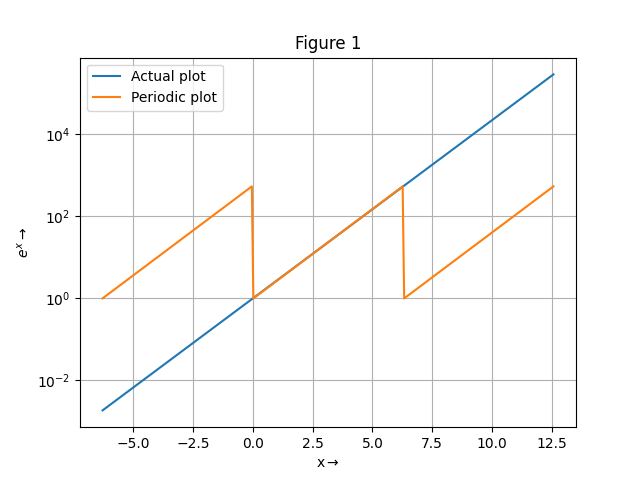
\includegraphics[width = 0.9\textwidth]{1a.png}
\caption{Semilog plot for $e^{x}$}
\end{figure} 
\newline
\newline
\newline
\newline
\newline
\newline
\newline
\newline
\newline
\newline
\newline
\newline
\newline
\newline
\begin{figure}[!tbh]
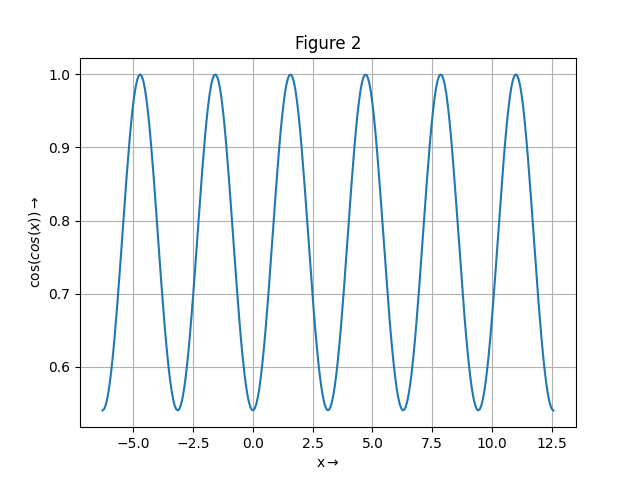
\includegraphics[width = 0.8\textwidth]{1b.png}
\caption{Plot for $cos(cos(x))$}
\end{figure} 


\section{Fourier Series Coefficients}

The first 51 Fourier series coefficients are obtained using the quad function.
A graph is plotted between the magnitude of coefficients and n in both semilog and loglog for both the functions in semilog and loglog scale
\begin{figure}[!tbh]
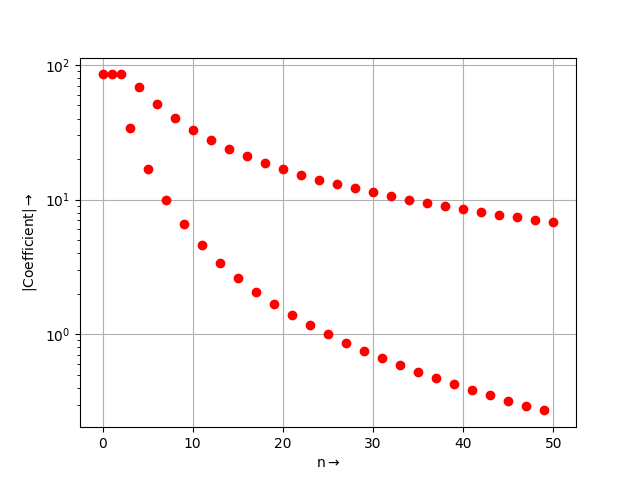
\includegraphics[width = 0.9\textwidth]{3a1.png}
\caption{Semilog plot of magnitude of coefficients for $e^{x}$}
\end{figure} 

\begin{figure}[!tbh]
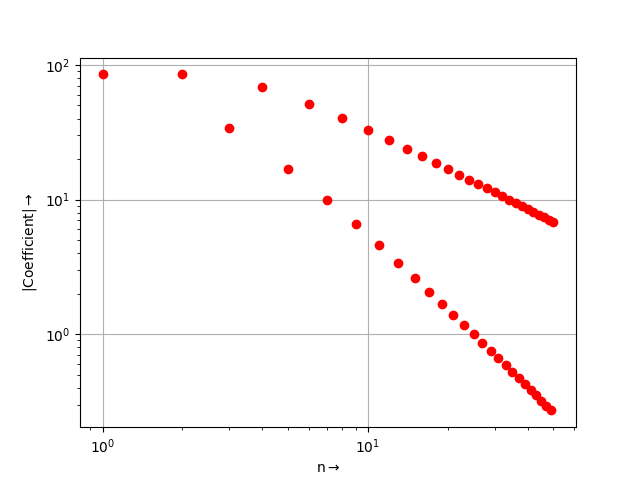
\includegraphics[width = 0.9\textwidth]{3a2.png}
\caption{Loglog plot of magnitude of coefficients for $e^{x}$}
\end{figure} 

\begin{figure}[!tbh]
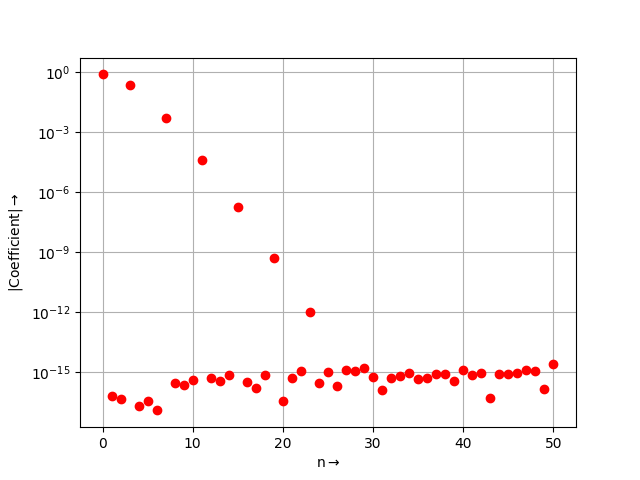
\includegraphics[width = 0.9\textwidth]{3b1.png}
\caption{Semilog plot of magnitude of coefficients for $cos(cos(x))$}
\end{figure} 

\begin{figure}[!tbh]
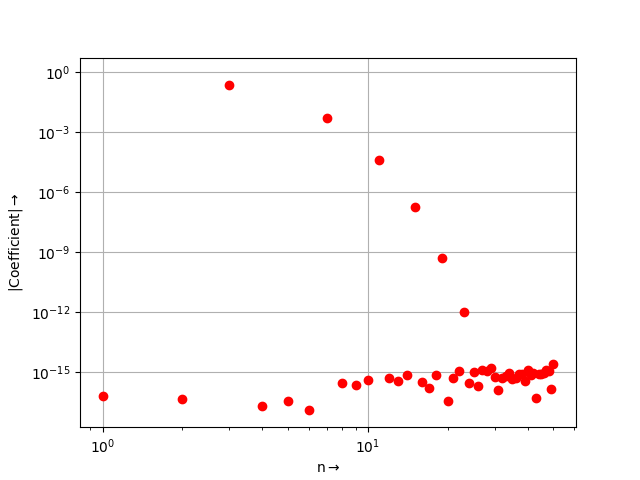
\includegraphics[width = 0.9\textwidth]{3b2.png}
\caption{Loglog plot of magnitude of coefficients for $cos(cos(x))$}
\end{figure} 

Clearly the bn coeeficients for coscos(x) are nearly zero as coscos(x) is an even function.
The magnitude of coefficients represents how much frequencies happen to be in the output.
So for $e^{x}$ it does not die quickly compared to coscos(x) as there is a discontinuity in periodic extension of $e^{x}$.
Loglog plot is linear for $e^{x}$ and as the coefficients decay with approx $1/n$ or $1/n^{2}$ 
Semilog plot is linear for coscos(x) as the coefficients decay exponentially with n

\section{Least Squares Approach}
The plot between the exact and approximation value of coefficients for both the functions in semilog and loglog are given below:
\begin{figure}[!tbh]
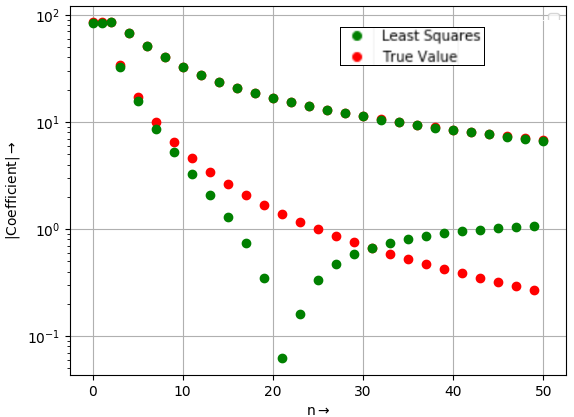
\includegraphics[width = 0.9\textwidth]{5a1.png}
\caption{Semilog plot of coefficients for $e^{x}$}
\end{figure} 

\begin{figure}[!tbh]
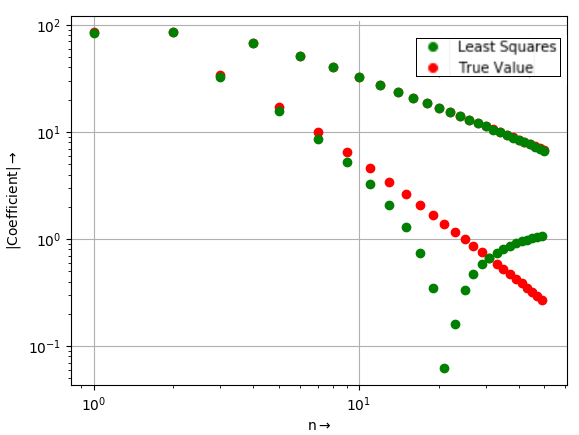
\includegraphics[width = 0.9\textwidth]{5a2.png}
\caption{Loglog plot of coefficients for $e^{x}$}
\end{figure} 

\begin{figure}[!tbh]
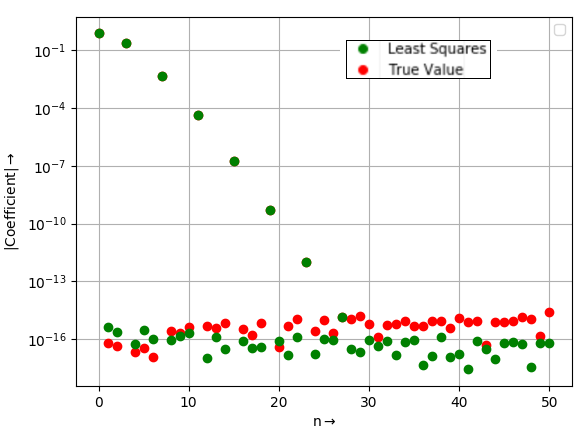
\includegraphics[width = 0.9\textwidth]{5b1.png}
\caption{Semilog plot of coefficients for $cos(cos(x))$}
\end{figure} 


\begin{figure}[!tbh]
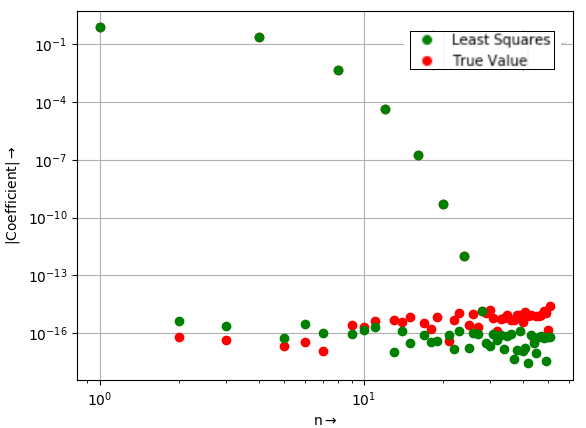
\includegraphics[width = 0.9\textwidth]{5b2.png}
\caption{Loglog plot of coefficients for $cos(cos(x))$}
\end{figure} 

As clearly expected coefficients of coscos(x) are in much closer compared to $e^{x}$ as the later have a discontinuity in its periodic 
extension resulting in need of higher sinusoids for a better representation.

The maximum deviation in the approximated and exact value of coefficients for the functions is given below:

Maximum deviation for $e^{x}$   : 1.3327308703353395

Maximum deviation for coscos(X) : 2.7586698812539523$e^{-15}$



\section{Function Approximation}
Plot between actual value of function and that obtained by multiplication of matrices A and c in the least squares approach to know the better estimate between them for both the functions is given below:
\newline
\newline
\newline
\newline
\newline
\newline
\newline\newline
\newline
\newline
\newline
\newline
\newline
\newline
\newline
\newline
\newline
\newline
\newline
\newline\newline
\newline
\newline
\newline
\newline
\newline
\newline
\newline
\begin{figure}[!tbh]
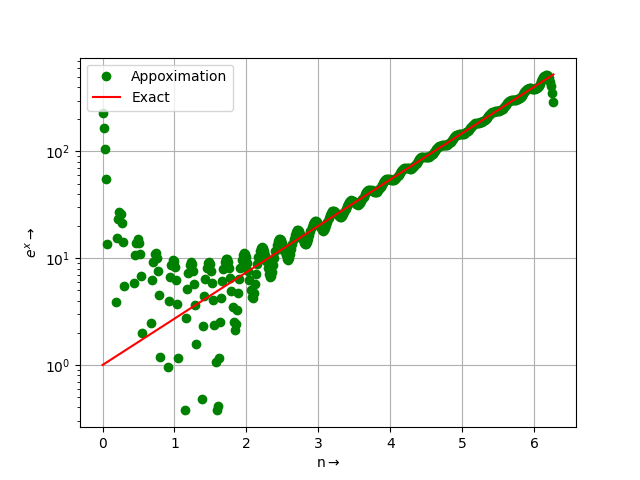
\includegraphics[width = 0.9\textwidth]{7a.png}
\caption{Semilog plots $e^{x}$ and its approx value}
\end{figure} 

\begin{figure}[!tbh]
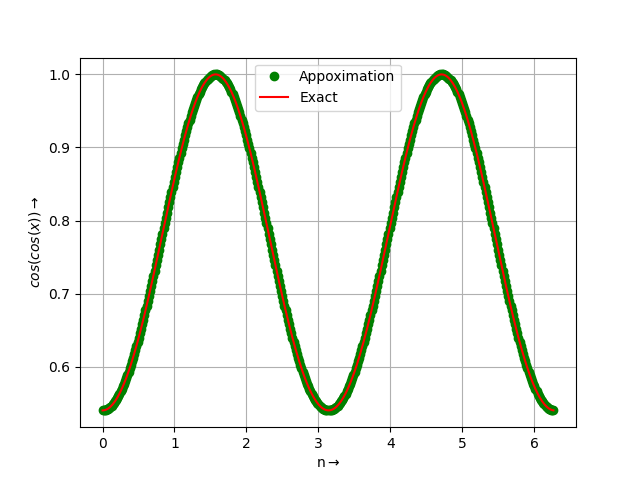
\includegraphics[width = 0.9\textwidth]{7b.png}
\caption{Plot of $cos(cos(x))$ and its approx value}
\end{figure} 


As expected there is a significant deviation in case of $e^{x}$ compared to coscos(x) where its almost same
\newline
\newline
\newline
\newline


\section{Conclusion}
Fourier series coefficients for the functions $e^{x}$ and coscos(x) were found in both direct integration and least squares approach.
The odd sinusoidal components for coscos(x) were zero as the function is itself an even function. 
There was a significant deviation in case of $e^{x}$ as there is a discontinuity in its periodic extension paving way to higher sinusoids for a better representation



\end{document}